\section{Ziel}
\label{sec:Ziel}
Im folgenden Experiment soll die Elektronenemmision durch Erwärmung einer Metalloberfläche untersucht werden. Dies wird als glühelektrischer Effekt bezeichnet. Dabei soll insbesondere die Temperaturabhängigkeit betrachtet, sowie die Austrittsarbeit des vorliegenden Metalles Wolfram bestimmt werden.

\section{Theorie}
\label{sec:theorie}

\subsection{Der Begriff der Austrittsarbeit}

Metalle weisen Kristallstrukturen auf. Das heißt, die nicht frei beweglichen Atome bilden ein Gitter, welches von freien Elektronen, welche als Leitungselektronen bezeichnet werden, umgeben ist. Näherungsweise kann angenommen werden, dass das Potential innerhalb dieses Gitters konstant ist, das sich um $\phi$ von dem im Außenraum vorliegenden Potential unterscheidet. Somit gilt das Potentialtopfmodell, welches in Abbildung \ref{fig:potentialtopf} dargestellt ist. Die Elektronen sind innerhalb des Metalles keinen Kräften ausgesetzt. Um aus dem Metall austreten zu können, muss ein Elektron die Potentialdifferenz überwinden. Die dazu aufzuwendende Energie wird als Austrittsarbeit bezeichnet. Sie beträgt
\begin{equation}
  W_\mathrm{A}= e \phi.
\end{equation}
Dabei ist $e$ die Elementarladung.

\begin{figure}
  \centering
  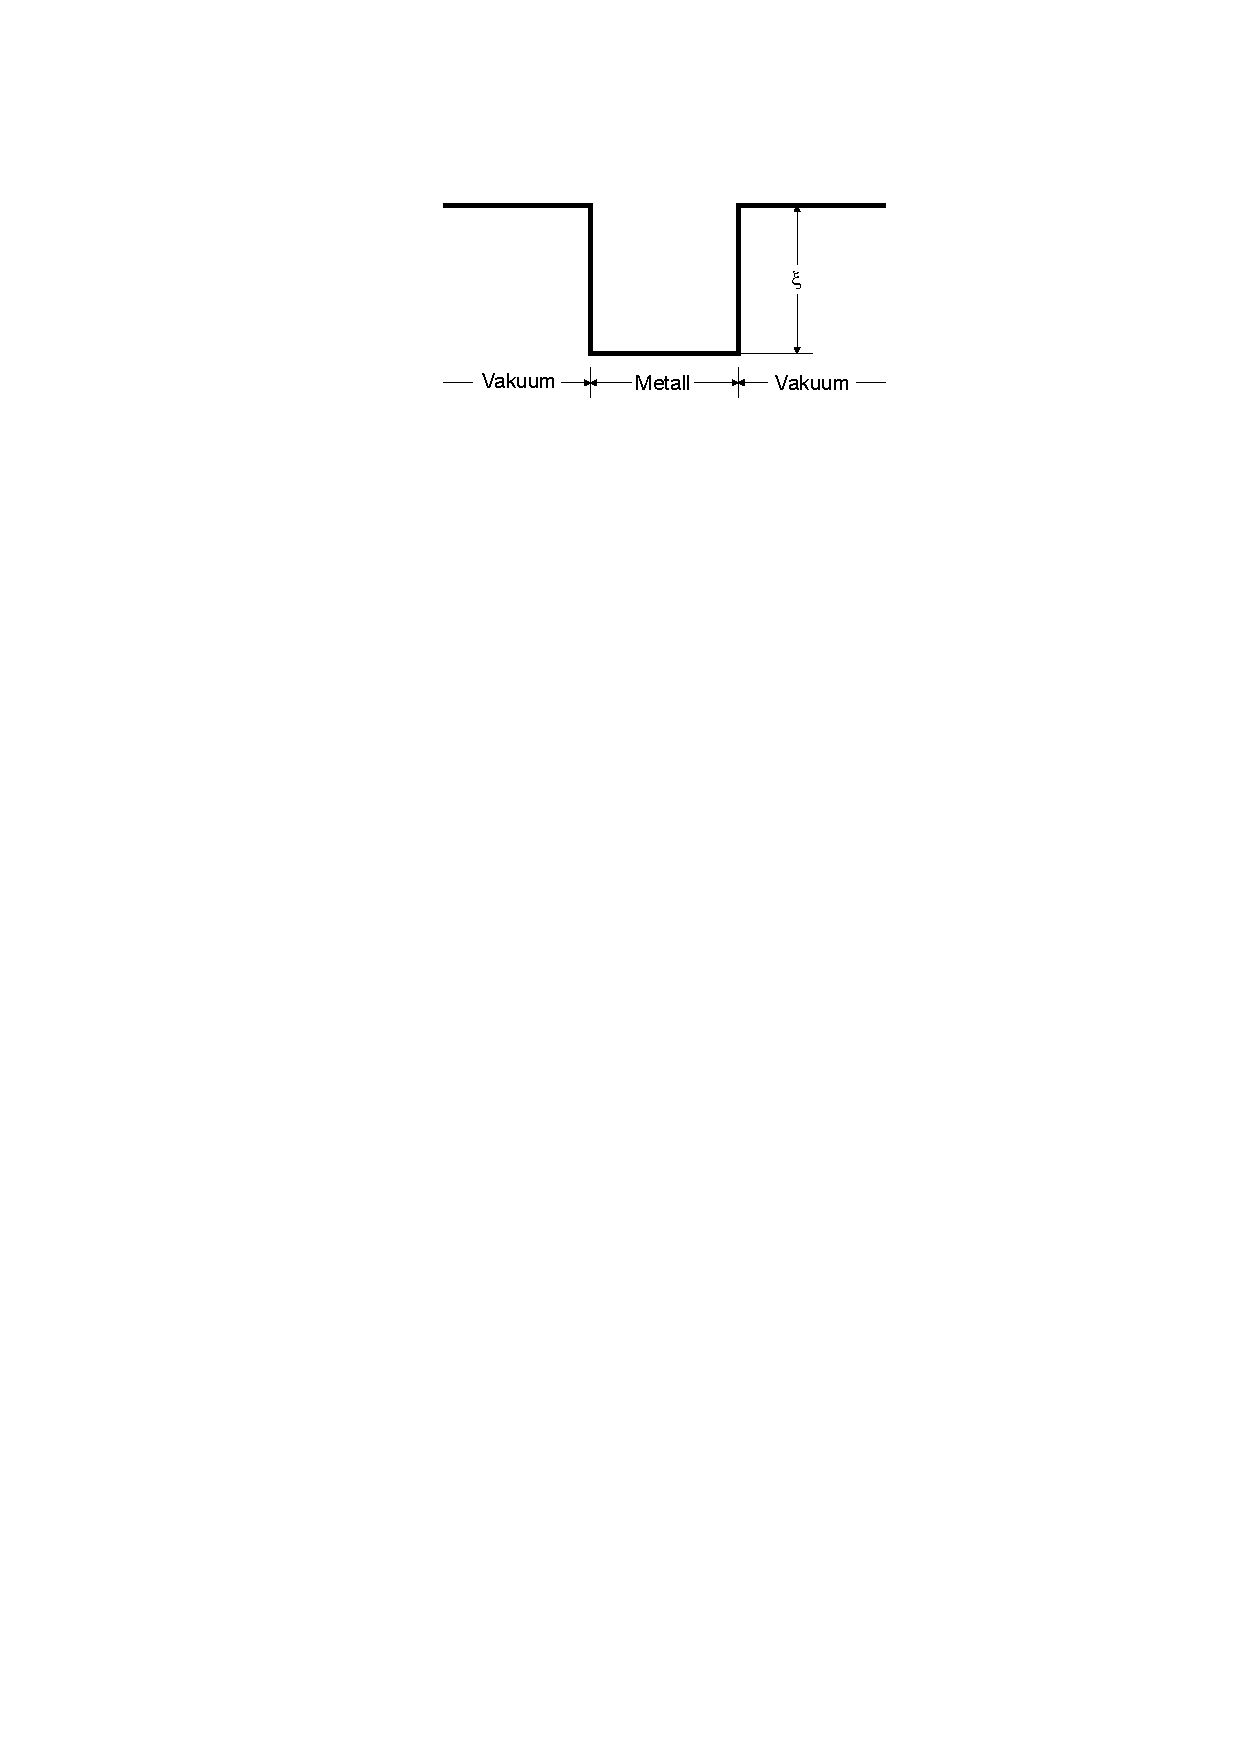
\includegraphics[scale=0.8]{content/potentialtopf.pdf}
\caption{Potentialtopf-Modell eines Metalles \cite{anleitung504}.}
  \label{fig:potentialtopf}
\end{figure}

\subsection{Die Kennlinie einer Hochvakuumdiode}
Um Wechselwirkungen der emittierten Elektronen mit Luftmolekülen zu vermeiden, wird das Experiment mit einer Hochvakuumdiode durchgeführt.

\begin{figure}
  \centering
  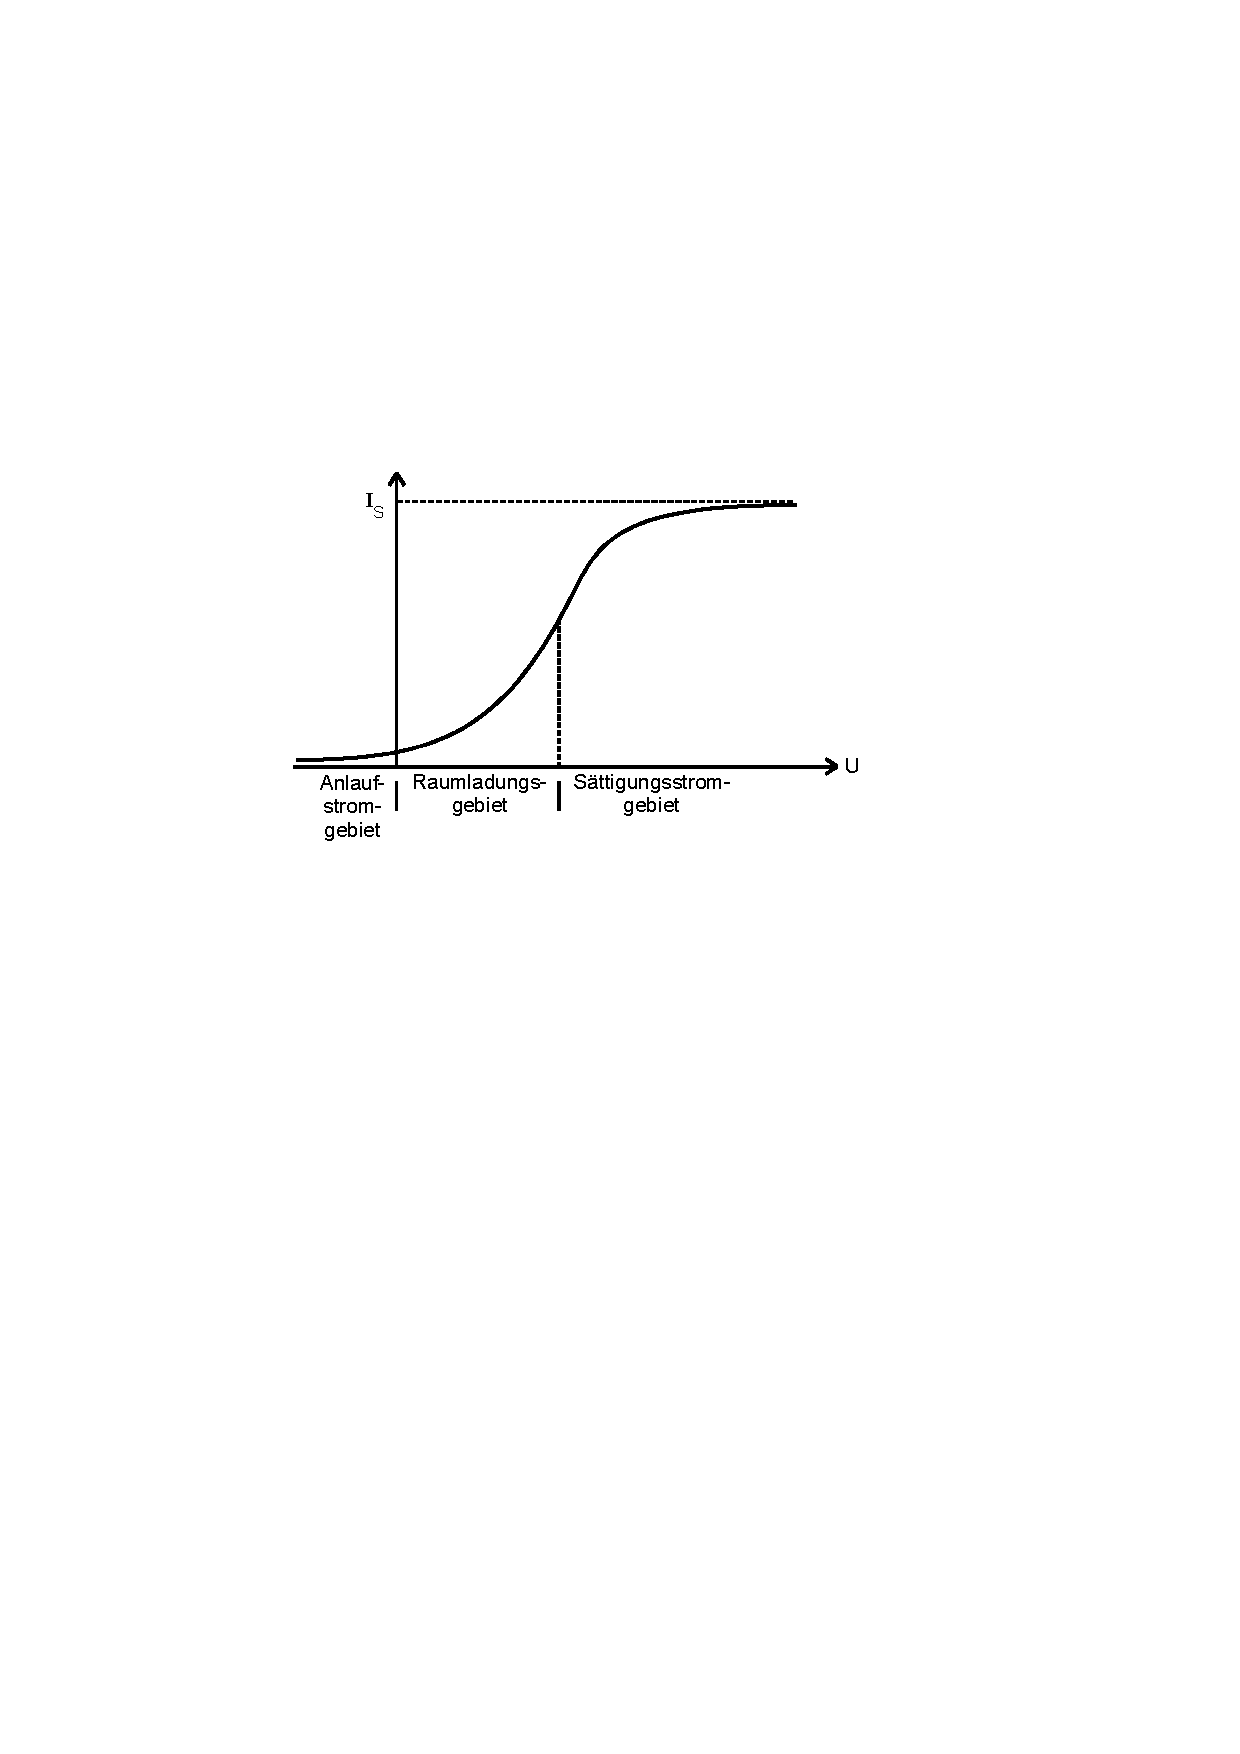
\includegraphics[scale=0.8]{content/kennlinie.pdf}
\caption{Kennlinie einer Hochvakuumdiode \cite{anleitung504}.}
  \label{fig:kennlinie}
\end{figure}

Abbildung \ref{fig:kennlinie} zeigt die Kennlinie einer Hochvakuumdiode, welche den Zusammenhang zwischen dem Anodenstrom $I_\mathrm{A}$ und und der von außen angelegten Spannung beschreibt. Sie besteht aus drei Bereichen, dem Anlaufstrom-, Raumladungs-, und Sättigungsstromgebiet, welche im folgenden erläutert werden.

\subsubsection{Anlaufstromgebiet}
Es ist zu beobachten, dass bei $U=0$ ein geringer Anodenstrom gemessen werden kann. Dieser ist auf die Eigengeschwindigkeit der Elekronen zurückzuführen.
Nach der Fermi-Diracschen Verteilungsfunktion, welche die Wahrscheinlichkeit für einen Energiezustand im thermischen Gleichgewicht angibt, existieren endlich viele Elektronen, die die Gegegenspannung überwinden können, was zu einem Anodenstrom führt.
Für die Stromdichte $j$ gilt in diesem Gebiet:
\begin{equation}
  j_\mathrm{A}(V)=C e^{-\frac{e V}{k_\mathrm{B}T}}.
\end{equation}
Dabei ist $C$ eine Konstante, $V$ das äußere Potential, $e$ die Elementarladung und $k_\mathrm{B}$ die Boltzmann-Konstante.

\subsubsection{Raumladungsgebiet}
Auf das Anlaufstromgebiet folgt das Raumladungsgebiet. Hier erreichen erst ab einer bestimmten Anodenspannung alle Elektronen die Anode. Dies kann durch die beschleunigte Bewegung der Elektronen von der Kathode zur Anode erklärt werden. Durch eben diese Beschleunigung ist die Raumladungsdichte $\rho$ nicht konstant, sondern abhängig vom Ort. Sie nimmt in Richtung der Anode ab, wie Abbildung \ref{fig:raumladung} zeigt. Die Raumladungsdichte beeimflusst den Verlauf der elektrischen Feldstärke $E$, was ebenfalls in Abbildung \ref{fig:raumladung} zu erkennen ist. Sie nimmt in Richtung der Anode zu.

\begin{figure}
  \centering
  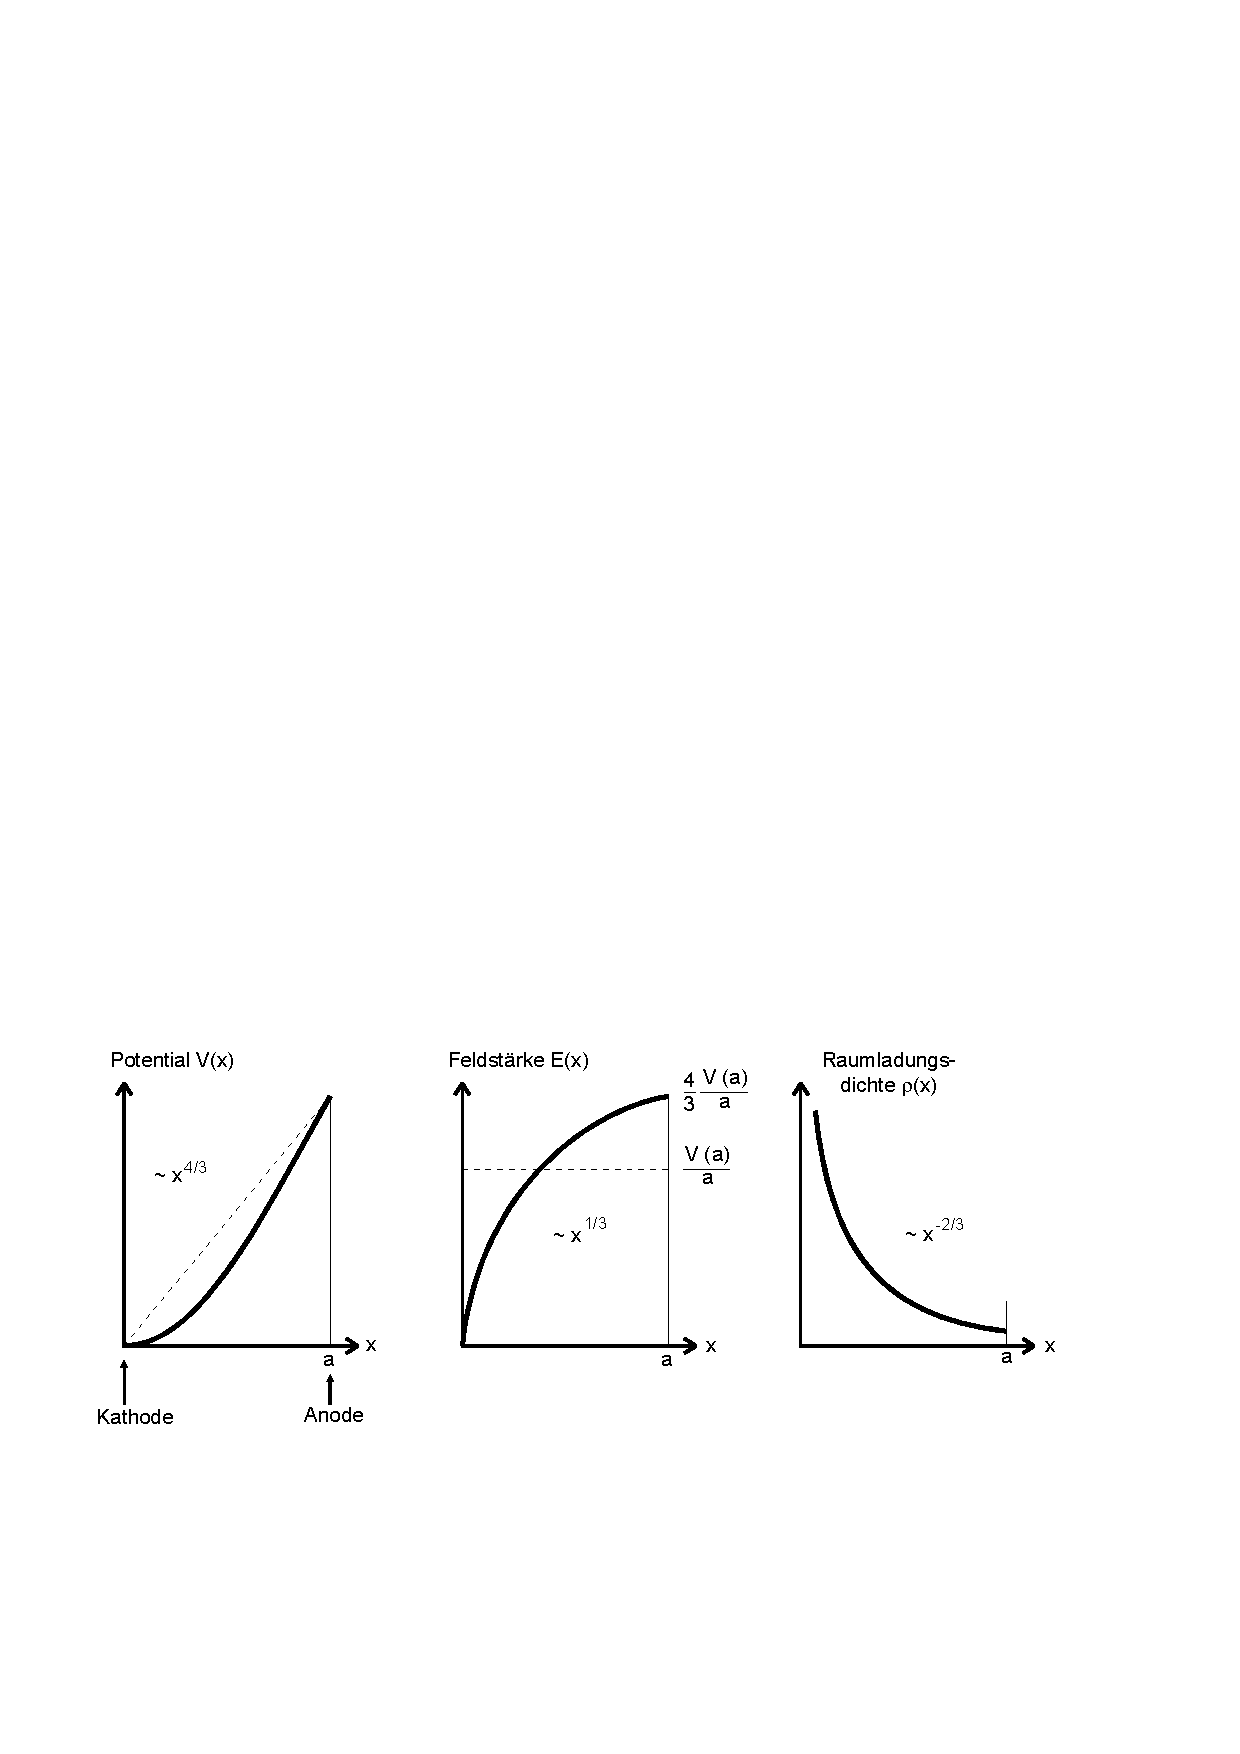
\includegraphics[scale=0.6]{content/raumladungsgebiet.pdf}
\caption{ Potential $V$, Feldstärke $E$  und Raumladungsdichte $\rho$ in Abhängigkeit vom Ort im Raumladungsgebiet \cite{anleitung504}.}
  \label{fig:raumladung}
\end{figure}

Es gilt das Langmuir-Schottkysche Raumladungsgesetz:
\begin{equation}
  j_\mathrm{R}=\frac{4}{9} \epsilon_0 \sqrt{\frac{2e}{m_0}}\frac{V^{\frac{3}{2}}}{a^2}
\end{equation}
mit $\epsilon_0$ als Dielektrizitätskonstante des Vakuums, $a$ als Ort der Anode.

\subsubsection{Sättigungsstromgebiet}
Im auf das Raumladungsgebiet folgende Sättigungsstromgebiet erreichen alle emittierten Elektronen die Anode. Es gilt die Richardson-Gleichung:
\begin{equation}
j_\mathrm{S}(T)=4\pi\frac{e m_0 k_\mathrm{B}^2}{h^3}T^2e^{\frac{-W_\mathrm{A}}{k_\mathrm{B}T}}
\end{equation}
Dabei ist $h$ das Plancksche Wirkungsquantum, $T$ die Temperatur und $W_\mathrm{A}$ die Austrittsarbeit für Elektronen.
